\documentclass{standalone}
\usepackage{tikz}

\begin{document}
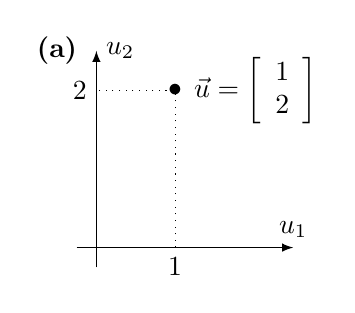
\begin{tikzpicture}
  \node at (-0.5, 2.5) {\bf (a)};
  \draw[-latex] (-0.25,0)--(2.5,0) node[above] {\(u_1\)};
  \draw[-latex] (0,-0.25)--(0,2.5) node[right] {\(u_2\)};
  \node at (1,2) {\(\bullet\)};
  \node[right] at (1,2) {\(\ \vec{u} =\left[\begin{array}{c} 1\\2\end{array}\right]\)};
  \draw[dotted] (1,0) -- (1,2) -- (0,2) node [left] {\(2\)};
  \node[below] at (1,0) {\(1\)};
\end{tikzpicture}
\hspace{0.25in}
\begin{tikzpicture}[scale=1.5]
  \node at (-0.5, 2.5) {\bf (b)};
  \draw[-latex] (-0.25,0)--(2.5,0) node[above] {\(u_1\)};
  \draw[-latex] (0,-0.25)--(0,2.5) node[right] {\(u_2\)};
  \draw[-latex,blue] (0,0) -- (1,2);
  \node[right] at (1,2) {\(\ \vec{u} =\left[\begin{array}{c} 1\\2\end{array}\right]\)};
  \draw[dotted] (1,0) -- (1,2) -- (0,2) node [left] {\(2\)};
  \node[below] at (1,0) {\(1\)};
\end{tikzpicture}
\end{document}
